 \documentclass[11pt, oneside]{article} 
\usepackage{geometry}
\geometry{letterpaper} 
\usepackage{graphicx}
	
\usepackage{amssymb}
\usepackage{amsmath}
\usepackage{parskip}
\usepackage{color}
\usepackage{hyperref}

\graphicspath{{/Users/telliott_admin/Tex/png/}}
% \begin{center} 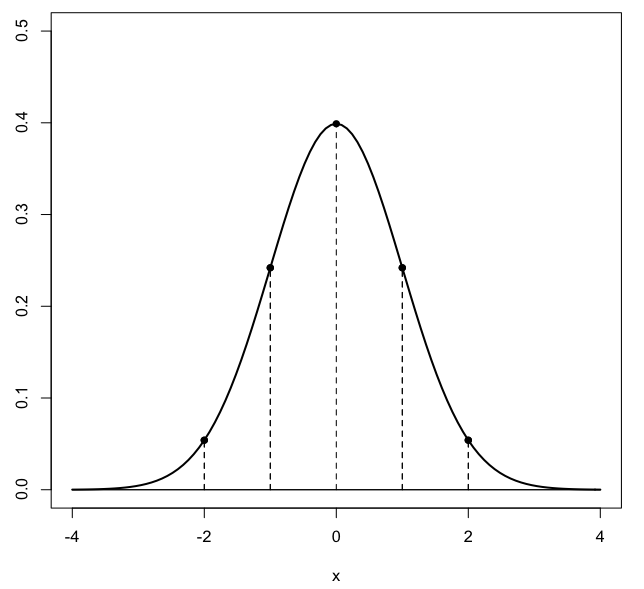
\includegraphics [scale=0.4] {gauss3.png} \end{center}

\title{Extreme Value Theorem}
\date{}

\begin{document}
\maketitle
\Large

\section{mini-max}

There is a maximum (and a minimum) value for $f$ on $[a,b]$

\subsection*{theorem}

If $f$ is continuous on $[a,b]$ then there is a number $y$ in $[a,b]$ such that $f(y) \ge f(x)$ for all $x$ in $[a,b]$.

\begin{center} 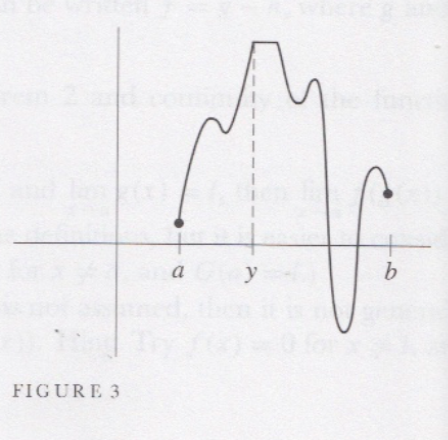
\includegraphics [scale=0.4] {spivak3.png} \end{center}

\subsection*{proof}





\subsection*{Bolzano-Weierstrass Theorem}

$\bullet$  Every bounded sequence has a convergent subsequence.

We proved this theorem in a previous section.  Now we use it to prove the following

\subsection*{theorem}

$\bullet$  Every continuous function on a closed bounded interval is bounded.

\url{www.tricki.org/article/How_to_use_the_Bolzano-Weierstrass_theorem}

We are given that $f$ is continuous.  For every $x \in [a,b]$ and for arbitrary $\epsilon > 0$ there exists $\delta > 0$ such that
\[  |y - x| < \delta \Rightarrow |f(y) - f(x)| < \epsilon \]

It is hard to see how to apply the theorem.

\subsection*{proof}

Suppose we consider the contrapositive.  Assume $f$ is unbounded, then prove that $f$ cannot be continuous.

If $f$ is unbounded, the assumption is that for every $C$ there exists $x \in [u,v]$ such that $f(x) > C$.  

If $C_1 > C_2$ and $|f(a)| > C_1$, then $|f(a)| > C_2$, so we can generate a sequence such that $|f(a_{n_k}) > n$ for every $n$.  

The sequence $(a_{n_k}) = C_1, C_2 \dots$ lies inside the closed and bounded interval $[u,v]$, so we can apply the BW theorem to it.

By the theorem, the subsequence must converge to some limit $a$.

The statement that $f$ is continuous at $a$ is equivalent to the statement that if $(b_m)$ is any sequence that converges to $a$ then $f(b_m)$ converges to $f(a)$. 

But we've already got a sequence that converges to $a$, namely the sequence $(a_{n_k})$. So if $f$ is continuous at $a$ then $f(a_{n_k})$ converges to $f(a)$. But that is impossible if $|f(a_{n_k})|>n_k$ for every $k$.  Thus $f$ cannot be continuous.

$\square$


\subsection*{theorem:  boundedness}

$\bullet$  The boundedness theorem states that a continuous function $f$ in the closed interval $[a,b]$ is bounded on that interval. That is, there exist real numbers $m$ and $M$ such that:

\[ m < f(x) < M \ \ \text{for all} \ x \in [a,b] \]

\subsection*{proof}

xxx

\subsection*{theorem:  extreme value}

$\bullet$  If a real-valued function $f$ is continuous in the closed and bounded interval $[a,b]$, then $f$ must attain a maximum and a minimum, each at least once.  

That is, there exist numbers $c$ and $d$ on $[a,b]$ such that
\[ f(d) \le f(x) \le f(c) \]
for all $x \in [a,b]$.

\subsection*{proof}

The set of $\{ \ y \in \mathbb{R}: y = f(x), \ \text{for} \ x \in [a,b] \ \}$ is a bounded set.  Hence it has a least upper bound.  Let $M = sup(f(x))$ on $[a,b]$.  

If $f(x)$ never equals the bound $M$, then $f(x) < M$ on $[a,b]$.  Therefore, $1/(M - f(x))$ is continuous on $[a,b]$.

However, because $M$ is the least upper bound, for arbitrary $\epsilon > 0$, there is always some $x$ in $[a,b]$ such that $M - f(x) < \epsilon$.  Hence $1/(M - f(x)) > 1/\epsilon$, which means that $1/(M - f(x))$ is not bounded.

Since every continuous function on $[a,b]$ is bounded, this contradicts the conclusion that $1/(M - f(x))$ is continuous on $[a,b]$.

Hence there must be some point $x$ in $[a,b]$ such that $f(x) = M$.







\end{document}